\documentclass[10pt,twocolumn]{article}
\usepackage[T1]{fontenc}
\usepackage{lmodern}
\usepackage[utf8]{inputenc}
\usepackage[letterpaper,top=0.75in,bottom=1in,left=0.68in,right=0.68in]{geometry}
\usepackage{setspace}
\usepackage{graphicx}
\usepackage{array}
\usepackage{tabularx}
\usepackage{booktabs}
\usepackage{caption}
\usepackage{enumitem}
\usepackage{hyperref}
\usepackage{soul}
\setlength{\columnsep}{0.17in}
\setlength{\parindent}{0.2in}
\captionsetup{font={small},labelfont=bf}
\sethlcolor{yellow}
\begin{document}
\twocolumn[
  \begin{center}
    {\fontsize{24}{28}\selectfont\textbf{EmotiTrack UDG (162/2025)}\par}\vspace{0.6ex}
    {\fontsize{11}{13}\selectfont Herrera Ramírez Johan Osvaldo, Escalante Maldonado Diego, Alexander Garcia Gonzalez, Cesar López Montes de Oca\par}\vspace{0.8ex}
    {\fontsize{10}{12}\selectfont\itshape CENTRO UNIVERSITARIO DE CIENCIAS EXACTAS E INGENIERÍAS, (CUCEI, UDG)\par}\vspace{0.6ex}
    {\fontsize{9}{11}\selectfont\texttt{johan.herrera4994@alumnos.udg.mx}\par}\vspace{0.3ex}
    {\fontsize{9}{11}\selectfont\texttt{diego.escalante0206@alumnos.udg.mx}\par}\vspace{0.3ex}
    {\fontsize{9}{11}\selectfont\texttt{garciaalexander22@ibm.com}\par}\vspace{1.0ex}
    {\fontsize{9}{11}\selectfont\texttt{cesar.lm@ibm.com}\par}\vspace{1.0ex}
    {\fontsize{9}{11}\selectfont\texttt{FIRMA DE VISTO BUENO DEL ASESOR}}\par
  \end{center}
  \vspace{1.5ex}
]
\noindent\textbf{\textit{Abstract}}\textbf{---} Este artículo presenta el desarrollo de EmotiTrack UDG, una aplicación modular diseñada para registrar, monitorear y analizar el estado emocional de estudiantes universitarios en el CUCEI. El sistema emplea cuestionarios breves basados en DASS-21 y análisis de datos para detectar niveles de estrés, ansiedad y depresión, permitiendo identificar patrones y cambios relevantes a lo largo del tiempo. La información recolectada se almacena de forma segura y se visualiza mediante informes y gráficos claros, facilitando la toma de decisiones institucionales orientadas a la prevención y el bienestar estudiantil. EmotiTrack integra prácticas de gestión ágil, arquitectura robusta y métodos de softcomputing para garantizar escalabilidad, seguridad y flexibilidad en el análisis. Los resultados buscan contribuir a la reducción de la deserción escolar y promover entornos académicos más saludables, con potencial de replicabilidad en otras instituciones educativas.

\noindent\textbf{\textit{Palabras clave}}\textbf{ -- }Bienestar emocional, estrés académico, DASS-21, análisis de datos, softcomputing, visualización, prevención, universidad, salud mental, modularidad.

\section*{I. INTRODUCCIÓN}
El estrés académico afecta significativamente el bienestar y rendimiento de los estudiantes universitarios, siendo una causa frecuente de ansiedad, depresión y deserción en el CUCEI de la Universidad de Guadalajara. Aunque existen aplicaciones internacionales para monitorear el estado emocional, es necesario contar con soluciones adaptadas al contexto local.

EmotiTrack UDG es una aplicación modular diseñada para registrar, monitorear y analizar el estado emocional de los estudiantes del CUCEI mediante cuestionarios breves y análisis de datos. Su objetivo es detectar niveles de estrés y cambios emocionales, proporcionando información útil a las autoridades para la toma de decisiones preventivas. El proyecto busca mejorar el bienestar estudiantil, reducir la deserción y facilitar la adopción de la herramienta en otras instituciones educativas.

\section*{II. Justificación del uso de DASS{-}21 frente a alternativas}

\textbf{Resumen.} Para un bot de entrevista por WhatsApp con \emph{check-ins semanales}, el DASS{-}21 ofrece un balance óptimo entre \emph{brevedad operativa} y \emph{propiedades psicométricas} sólidas. La evidencia empírica muestra que el DASS{-}21 mantiene alta confiabilidad y validez de constructo, presenta una estructura factorial más “limpia” que el DASS{-}42 y permite la equivalencia práctica de puntajes al duplicar las puntuaciones crudas para comparabilidad con normas del instrumento completo~[1].

\subsubsection*{Validez y confiabilidad}
El DASS{-}21 exhibe \textbf{elevadas consistencias internas} para Depresión, Ansiedad, Estrés y la escala Total, y \textbf{validez de constructo} respaldada por análisis factorial confirmatorio (AFC) en muestras amplias de población general. Asimismo, se han publicado \textbf{datos normativos específicos} para DASS{-}21 que facilitan la interpretación de resultados a nivel individual y grupal~[1].

\subsubsection*{Comparación con DASS{-}42}
Estudios que comparan directamente DASS{-}21 con DASS{-}42 reportan que la versión corta presenta una \textbf{estructura factorial más clara} y evita ítems problemáticos de la versión larga, sin sacrificar la diferenciación entre dimensiones de depresión, ansiedad y estrés~[1]. Además, \textbf{duplicar los puntajes crudos} de DASS{-}21 ofrece valores \emph{muy similares} a los del DASS{-}42, lo que habilita la continuidad con criterios y puntos de referencia previamente establecidos~[1].

\subsubsection*{Implicaciones para analítica y \emph{data mining}}
Para \textbf{minería de datos} y análisis semanal (EDA, \emph{feature engineering}, \emph{clustering} y modelos interpretables) el DASS{-}21 reduce \textbf{carga de respuesta} y \textbf{fatiga del participante}, aumentando la probabilidad de \emph{adhesión} en contextos de mensajería móvil. La brevedad con adecuada fidelidad psicométrica facilita \textbf{series temporales semanales} de mayor completitud, mejora la \textbf{calidad de datos} para algoritmos (p.\,ej., K{-}Means/DBSCAN, CART) y favorece la detección de \emph{patrones} y \emph{hotspots} por materia/periodo académico.

\subsubsection*{Limitaciones y medidas de mitigación}
El DASS{-}21 es un \textbf{tamizaje dimensional} y no un diagnóstico clínico. Se recomienda: (i) incluir mensajes de \emph{disclaimer} en el bot, (ii) vigilar \emph{drift} y \emph{missingness} en los datos semanales, y (iii) acompañar con rutas de derivación cuando se observen puntajes elevados persistentes. Estas prácticas preservan la \textbf{utilidad preventiva} y la \textbf{responsabilidad ética} del sistema.

\section*{III. DESCRIPCIÓN DEL DESARROLLO DEL PROYECTO MODULAR}
Todos los párrafos deben tener indentado o tabulaciones en la primera línea. También, todos los párrafos deben estar alineados de forma justificada y hacia la izquierda.

\subsection*{A. Tipo de letra fuente para el documento}
La totalidad del documento se debe escribir usando Times New Roman o equivalente. Otros tipos de fuente serán utilizados solamente cuando sea requerido para casos especiales.

Los tamaños de fuente se incluyen en la Tabla~\ref{tab:format-sizes}.

\subsection*{B. Título y detalles del autor(es)}
El título debe estar en fuente tamaño 24 puntos. Los nombres de los autores en tamaño de 11 puntos. El nombre de la universidad y departamentos en letra tamaño 10 puntos y cursiva y finalmente los correos electrónicos en tamaño 9 puntos con una fuente tipo Courier.

\begin{table}[t]
  \centering
  \caption{Tamaños de formato de texto}
  \label{tab:format-sizes}
  \begin{tabularx}{\linewidth}{@{}>{\raggedright\arraybackslash}p{0.16\linewidth}*{3}{>{\raggedright\arraybackslash}X}@{}}
    \toprule
    \multicolumn{1}{c}{Tamaño} & \multicolumn{3}{c}{Apariencia (en Times New Roman o Times)} \\
    \cmidrule(l){1-1}\cmidrule(l){2-4}
     & Regular & Negrita & Cursiva \\
    \midrule
    8 & Contenidos de tablas\\Título de figuras\\Referencias a objetos & Negrita & Cursiva \\
    9 & Direcciones de correo electrónico\\(usar fuente Courier)\\Cuerpo del proyecto & Negrita\\Cuerpo del abstract & Cursiva \\
    10 & Subtítulos & Negrita & Cursiva \\
    11 & Nombre del autor & Negrita & Cursiva \\
    24 & Título del proyecto & & \\
    \bottomrule
  \end{tabularx}
\end{table}

El título, autores, universidad y correos deben estar en el encabezado de la primera página, en una sola columna que abarca las dos columnas inferiores. Todo este texto debe estar centrado.

Cada palabra en un título debe iniciar con mayúscula, excepto palabras menores como: “a”, “de”, “y”, “desde” entre otras.

Para evitar confusiones, el apellido de cada autor debe ser escrito siempre.

\subsection*{C. Encabezados de sección}
Cada sección deberá dividirse como máximo en 3 niveles de sub-secciones. Todo subtítulo deberá tener letra de tamaño 10 puntos y cada palabra en el título deberá iniciar con mayúscula excepto las palabras menores como se indicó en la sección II.B.

Observe en la línea anterior cómo se hace una referencia a otra sección del documento, usando el número de título III y el de subtítulo B.

Cuando necesite crear varios niveles de sección en el documento (título, subtítulo, etc.) utilice estas normas:
\begin{enumerate}[leftmargin=*,label=\roman*.]
  \item \textit{Primer nivel}: El primer nivel corresponde al de título, por tanto, debe estar centrado, indexado con números romanos y todas las letras en mayúscula con la primera letra de las palabras mayores en mayor tamaño.
  \item \textit{Segundo nivel}: Un segundo nivel corresponde al subtítulo. Deben estar numerados usando letras seguidas por un punto y alineados a la izquierda. El tipo de letra es de 10 puntos y en cursiva.
  \item \textit{Tercer nivel}: Un tercer nivel es como este que está leyendo. Utiliza letra cursiva de 10 puntos enlistados con números arábigos seguidos por un paréntesis. El cuerpo del ítem debe estar inmediatamente después del encabezado, sin saltos de línea.
\end{enumerate}

\subsection*{D. Figuras y tablas}
Las figuras y tablas deben estar centradas en la columna. Si la figura es muy larga, se puede extender hasta ocupar el espacio de las dos columnas. Cualquier figura o tabla que se extienda más de una columna, pero no ocupe el espacio de las dos columnas, se deberá mostrar centrada en la página y deberá estar siempre en la parte superior o inferior de la página.

Los gráficos deben estar en color, de preferencia utilice colores estándar de manera que puedan ser reproducidos en cualquier sistema. Por colores estándar se entienden rojo, azul, verde, amarillo. Trate de evitar colores complejos como azul claro combinado con azul más fuerte porque podrían confundirse.

Utilice colores sólidos que resalten sobre el fondo de la figura para mejorar el contraste.

Toda figura debe acompañarse de un título en letra de tamaño de 8 puntos, que inicia con la abreviatura “Fig.” para indicar “Figura” y un número de secuencia.

El nombre de la figura debe tener mayúscula solamente en la primera palabra, independientemente de si se trata de una palabra mayor o menor.

El nombre de la figura se utiliza centrado en la columna, o página si la figura se extiende fuera de la columna. Si la descripción se extiende más de una línea, se debe mostrar de forma justificada, como en la Fig.~\ref{fig:solid-colors}.

\begin{figure}[t]
  \centering
  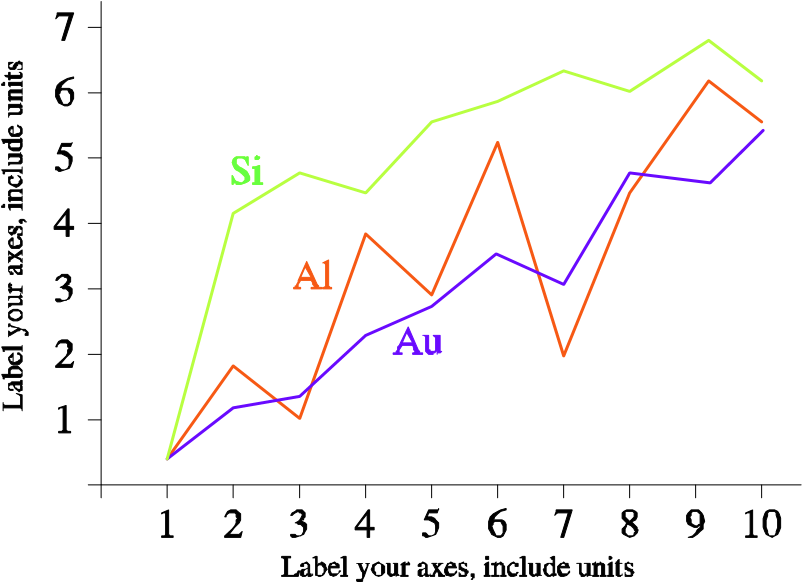
\includegraphics[width=0.75\columnwidth]{../img/image3.png}
  \caption{El ejemplo de un gráfico con colores sólidos que resaltan sobre el fondo blanco.}
  \label{fig:solid-colors}
\end{figure}

La Fig.~\ref{fig:low-res} es un ejemplo de una imagen importada al documento. En estos casos, asegúrese de utilizar la resolución adecuada, de manera que la figura se pueda apreciar con claridad en el documento.

No utilice figuras de resolución pobre porque empobrece la calidad del proyecto.

Cuando inserte una figura, asegúrese de verificar lo siguiente:
\begin{itemize}[leftmargin=*]
  \item los colores contrastan adecuadamente,
  \item la imagen es clara,
  \item cualquier texto en la imagen se puede leer claramente.
\end{itemize}

La Fig.~\ref{fig:low-res} muestra un caso donde la resolución no es adecuada, mientras que la Fig.~\ref{fig:good-res} muestra una mejor adaptación de la misma figura.

\begin{figure}[t]
  \centering
  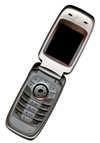
\includegraphics[width=0.55\columnwidth]{../img/image1.jpg}
  \caption{Ejemplo de figura con baja resolución}
  \label{fig:low-res}
\end{figure}

\begin{figure}[t]
  \centering
  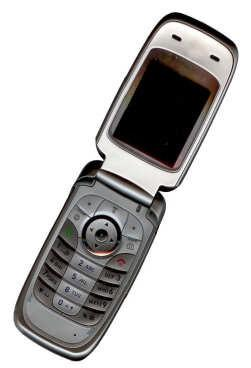
\includegraphics[width=0.53\columnwidth]{../img/image2.jpg}
  \caption{Ejemplo de figura con buena resolución}
  \label{fig:good-res}
\end{figure}

\subsection*{E. Títulos de tablas}
Las tablas deben tener un título con letra mayúscula de 8 puntos, centrado en la columna y con letra más grande en el inicio de cada palabra mayor. Antes de la línea del título, se incluye una línea centrada donde se usa la palabra “Tabla” seguida de la numeración de la tabla usando números romanos.

\subsection*{F. Números de página, encabezados y pie de página}
Estos tres elementos no deben ser utilizados.

\subsection*{G. Hiper-vínculos y accesos directos}
Cualquier hiper-vínculo o referencia a Internet debe escribirse por completo. Es decir, escribir el URL completo de la ubicación del recurso en lugar de dejar accesos directos.

Las referencias se escriben usando fuente regular igual que el resto del proyecto.

\subsection*{H. Referencias bibliográficas}
El encabezado de la sección de referencias debe seguir las normas del nivel “título” sin embargo, no debe tener numeración.

Todas las referencias se hacen en letra de 8 puntos.

Utilice cursiva para distinguir los diferentes campos de la referencia. Utilice los ejemplos adjuntos en este documento.

Todas las referencias están numeradas con números arábigos consecutivos que inician en 1 y siempre están encerrados en paréntesis cuadrados (p.e. [1]).

Si en el cuerpo del proyecto hace referencia a alguna de estas referencias, utilice solamente los paréntesis cuadrados y el número correspondiente. Nunca use términos como “ver referencia [4]”, en su lugar use “ver [4]”.

Si son varias referencias juntas, sepárelas con comas.

Las referencias cambian según el tipo de fuente.

Los ejemplos enumerados en la sección de referencias de este documento incluyen:
\begin{enumerate}[leftmargin=*,label=\alph*.)]
  \item ejemplo de un libro [1]
  \item ejemplo de un libro parte de una serie [2]
  \item ejemplo de otro artículo de revista [3]
  \item ejemplo de un artículo de conferencia [4]
  \item ejemplo de una patente [5]
  \item ejemplo de un sitio web [6]
  \item ejemplo de una página de un sitio web [7]
  \item ejemplo de un manual [8]
  \item ejemplo de una hoja de datos [9]
  \item ejemplo de una tesis [10]
  \item ejemplo de un reporte técnico [11]
  \item ejemplo de un estándar [12]
\end{enumerate}

\subsection*{Módulo Gestión de la tecnología de información}
Este módulo enmarca la \textbf{planificación, gobierno y operación} del proyecto modular. Define cómo se gestionan recursos, riesgos, calidad y seguridad para entregar valor con evidencia. En este proyecto se adopta \textbf{Scrum} (sprints, backlog, revisiones, DoD) con responsabilidades definidas: Johan (bot e integración) y Diego (analítica con Polars). Se gestionan \textbf{requisitos} para entrevistas \textbf{semanales} por WhatsApp basadas en DASS{-}21, \textbf{datos} (consentimiento, minimización, seudonimización, control de acceso y retención), \textbf{calidad y documentación} (reporte LaTeX, referencias IEEE, versionamiento, CI/CD), y \textbf{seguridad} (gestión de secretos, cifrado en tránsito y en reposo, RBAC). 

\subsection*{Módulo Sistemas robustos, paralelos y distribuidos}
Este módulo vincula la \textbf{arquitectura técnica} con la necesidad de disponibilidad, escalabilidad y tolerancia a fallos. La solución integra \textbf{WhatsApp Business Cloud API} mediante webhooks, un servicio de orquestación para envío/recepción de mensajes, \textbf{colas de mensajes} para desacoplar e implementar reintentos/backoff, y \textbf{workers} paralelos para procesar respuestas y persistir en la base de datos. Se emplea \textbf{Docker} y despliegues en nube (p.\,ej., Azure/AWS), con estrategias blue/green o rolling. Los \textbf{jobs semanales} de analítica usan \textbf{Polars} (ejecución perezosa y paralela) para EDA y agregaciones. La robustez se refuerza con timeouts, circuit breakers, idempotencia y DLQ; la \textbf{observabilidad} con logging estructurado, métricas y trazas distribuidas (SLO: disponibilidad $\geq$ 99\%, p95 $<$ 1\,s en webhook). Se contemplan respaldos, restauración ensayada e infraestructura como código.

\subsection*{Módulo Justificación de Cómputo Flexible (softcomputing)}
El proyecto aplica \textbf{métodos flexibles} para manejar variabilidad y ruido en datos de bienestar emocional. Se utiliza \textbf{DASS{-}21} con cálculo estandarizado de subescalas (depresión, ansiedad, estrés) en cortes \textbf{semanales}, validando completitud y rangos. La \textbf{ingeniería de características} incorpora contexto académico (materias, semanas de parciales/entregas), patrones de respuesta y cambios abruptos. Para descubrir \textbf{patrones de riesgo y evolución} se emplean \textbf{clustering} (K{-}Means/DBSCAN) y modelos \textbf{interpretables} tipo \textbf{CART} para reglas y umbrales trazables. La validación incluye CV, análisis de drift e interpretabilidad, con salvaguardas éticas (no diagnóstico clínico, uso para prevención). Los hallazgos se comunican en \textbf{tableros} (Streamlit/Gradio) que muestran tendencias semanales, clusters y hotspots por materia/fecha para apoyar decisiones institucionales.

\section*{IV. RESULTADOS OBTENIDOS DEL PROYECTO}
El propósito de esta sección es resumir los principales resultados discutidos a lo largo del proyecto. Recuerde manejar las conclusiones como enunciados cortos fundamentados en la teoría y los objetivos planteados.

Los resultados deben presentarse en el orden lógico y sucesivo en que fueron encontrados, de forma que sean comprensibles y coherentes.

Los resultados deben describir dos temas claves:

1) Expresar los objetivos reales alcanzados con el proyecto modular al término de su desarrollo.

2) Presentar su relación con la solución planteada.

(Esta sección debe ser escrita utilizando los verbos en pasado)

Esta sección no tiene requisitos especiales de formato.

\section*{V. CONCLUSIONES Y TRABAJO A FUTURO}
El propósito de esta sección es resumir los principales resultados discutidos a lo largo del proyecto. Recuerde manejar las conclusiones como enunciados cortos fundamentados en la teoría y los objetivos planteados.

Esta sección no tiene requisitos especiales de formato.

\section*{RECONOCIMIENTOS}
Esta sección sigue el formato regular del resto del documento. La única observación es notar que el título no está numerado.

En esta sección se agregan agradecimientos a personas que colaboraron en el proyecto pero que no figuran como autores del proyecto.

\section*{REFERENCIAS}
\begin{thebibliography}{12}
  \bibitem{henrycrawford2005}
  J.~D. Henry and J.~R. Crawford, ``The short-form version of the Depression Anxiety Stress Scales (DASS{-}21): Construct validity and normative data in a large non-clinical sample,'' \emph{British Journal of Clinical Psychology}, vol.~44, no.~2, pp.~227--239, Jun. 2005, doi: 10.1348/014466505X29657.
\end{thebibliography}
\end{document}
